\documentclass[conference]{IEEEtran}
\usepackage{caption}
\usepackage{graphicx}
\graphicspath{ {images/} }
\usepackage[rightcaption]{sidecap}
\usepackage{wrapfig}
\usepackage{float}

\title{Analysis of how workplace factors impact mental health: conclusions from employee research}
\author{Maja Placek\\
Applied Computer Science\\
Wrocław University of Science and Technology\\
266538@student.pwr.edu.pl }

\begin{document}
\maketitle

\section{Introduction}
With the growing awareness of the impact of mental health state on an employee and their productivity, the topic of how workplace influences mental well-being seems to be gaining increasing interest. In recent years, factors like company size, remote work-style, mental health benefits have drawn particular attention. 

In this report I am going to analyze correlations between workplace-related factors and outcomes concerning employees mental health state. To achieve this, I will utilize the results of a survey available at the following website: \cite{dataset}

This way, I will attempt to identify means in which employers could promote mental health of their employees and consequently improve overall atmosphere in the company.
\section{Data set and its processing}

\subsection{Data set}
The data set was obtained from the website \cite{dataset}. It includes results from a survey that measures attitudes towards mental health and frequency of mental health disorders in the workplace.\\

The survey included 27 questions:
\begin{enumerate}
    \item Timestamp
    \item Age
    \item Gender
    \item Country
    \item state: If you live in the United States, which state or territory do you live in?
    \item self\_employed: Are you self-employed?
    \item family\_history: Do you have a family history of mental illness?
    \item treatment: Have you sought treatment for a mental health condition? 
    \item work\_interfere: If you have a mental health condition, do you feel that it interferes with your work?
    \item no\_employees: How many employees does your company or organization have?
    \item remote\_work: Do you work remotely (outside of an office) at least 50\% of the time?
    \item tech\_company: Is your employer primarily a tech company/organization?
    \item benefits: Does your employer provide mental health benefits?
    \item care\_options: Do you know the options for mental health care your employer provides?
    \item wellness\_program: Has your employer ever discussed mental health as part of an employee wellness program?
    \item seek\_help: Does your employer provide resources to learn more about mental health issues and how to seek help?
    \item anonymity: Is your anonymity protected if you choose to take advantage of mental health or substance abuse treatment resources?
    \item leave: How easy is it for you to take medical leave for a mental health condition?
    \item mental\_health\_consequence: Do you think that discussing a mental health issue with your employer would have negative consequences?
    \item phys\_health\_consequence: Do you think that discussing a physical health issue with your employer would have negative consequences?
    \item coworkers: Would you be willing to discuss a mental health issue with your coworkers?
    \item supervisor: Would you be willing to discuss a mental health issue with your direct supervisor(s)?
    \item mental\_health\_interview: Would you bring up a mental health issue with a potential employer in an interview?
    \item phys\_health\_interview: Would you bring up a physical health issue with a potential employer in an interview?
    \item mental\_vs\_physical: Do you feel that your employer takes mental health as seriously as physical health?
    \item obs\_consequence: Have you heard of or observed negative consequences for coworkers with mental health conditions in your workplace?
    \item comments: Any additional notes or comments
\end{enumerate}

\subsection{Pre-processing}

\subsubsection{Data cleaning}
\begin{itemize}
    \item Column names were changed into lower case.
    \item Age: Entries with invalid values (-29, 5, 329 etc.) were discarded. The data set was filtered to include only individuals within the age range of 18 to 70 years.
    \item Gender: The gender variable values were narrowed down to [Female, Male, Other].
    \item Timestamp: entries were filtered to include only those from year 2014 (due to very low variance).
\end{itemize}

\subsubsection{Dropped columns}
I have decided to drop the following columns due to specified problems:
\begin{itemize}
    \item timestamp: low variance
    \item country: low variance
    \item state: correlated with country
    \item comments: unusable data
\end{itemize}

\subsubsection{Dealing with missing data}
\begin{itemize}
    \item self\_employed: Nan entries were dropped because the number of them was negligible and it would be difficult to interpret missing values.
    \item work\_interfere: Empty entries were substituted with 'Unknown'.
\end{itemize}

\subsubsection{Data encoding}
The encoding technique used in the analysis is a combination of label encoding, manual mapping and one hot encoding.
The variables 'work\_interfere', 'no\_employees', and 'leave' are encoded using label encoding based on a predefined order or ranking. Each unique category within these variables was assigned a numerical value based on a predefined order or ranking. For example, in the 'work\_interfere' variable, the categories 'Unknown' and 'Never' were encoded as 0, 'Rarely' as 1, 'Sometimes' as 2, and 'Often' as 3. Similarly, the 'no\_employees' variable was encoded with numerical values ranging from 0 to 5, representing different employee count ranges.
One hot encoding technique was used to encode gender variable.

\onecolumn
\subsection{Exploratory Data Analysis}

\begin{table}[h]
\centering
\begin{tabular}{|l|r|r|}
\hline
                  & raw data & after pre-processing \\ \hline
number of entries & 1259     & 1163                 \\ \hline
number of columns & 27       & 25                   \\ \hline
\end{tabular}
\caption{Data before and after pre-processing}
\label{tab:raw-normalized}
\end{table}

\begin{table}[h]
\centering
\begin{tabular}{|l|l|l|l|}
\hline
                            & 0                   & 1                   & 2                   \\ \hline
timestamp                   & 2014-08-27 11:29:31 & 2014-08-27 11:29:37 & 2014-08-27 11:29:44 \\ \hline
age                         & 37                  & 44                  & 32                  \\ \hline
gender                      & Female              & M                   & Male                \\ \hline
country                     & United States       & United States       & Canada              \\ \hline
state                       & IL                  & IN                  & NaN                 \\ \hline
self\_employed              & NaN                 & NaN                 & NaN                 \\ \hline
family\_history             & No                  & No                  & No                  \\ \hline
treatment                   & Yes                 & No                  & No                  \\ \hline
work\_interfere             & Often               & Rarely              & Rarely              \\ \hline
no\_employees               & 6-25                & More than 1000      & 6-25                \\ \hline
remote\_work                & No                  & No                  & No                  \\ \hline
tech\_company               & Yes                 & No                  & Yes                 \\ \hline
benefits                    & Yes                 & Don't know          & No                  \\ \hline
care\_options               & Not sure            & No                  & No                  \\ \hline
wellness\_program           & No                  & Don't know          & No                  \\ \hline
seek\_help                  & Yes                 & Don't know          & No                  \\ \hline
anonymity                   & Yes                 & Don't know          & Don't know          \\ \hline
leave                       & Somewhat easy       & Don't know          & Somewhat difficult  \\ \hline
mental\_health\_consequence & No                  & Maybe               & No                  \\ \hline
phys\_health\_consequence   & No                  & No                  & No                  \\ \hline
coworkers                   & Some of them        & No                  & Yes                 \\ \hline
supervisor                  & Yes                 & No                  & Yes                 \\ \hline
mental\_health\_interview   & No                  & No                  & Yes                 \\ \hline
phys\_health\_interview     & Maybe               & No                  & Yes                 \\ \hline
mental\_vs\_physical        & Yes                 & Don't know          & No                  \\ \hline
obs\_consequence            & No                  & No                  & No                  \\ \hline
comments                    & NaN                 & NaN                 & NaN                 \\ \hline
\end{tabular}
\captionsetup{justification=centering, belowskip=10pt}
\caption{Representative data sample}
\label{tab:my-table}
\end{table}
Due to the low variance in 'Country' variable I have decided to discard this column. Consequently 'state' variable was also dropped.
\begin{wrapfigure}{r}{\textwidth}
    \centering
    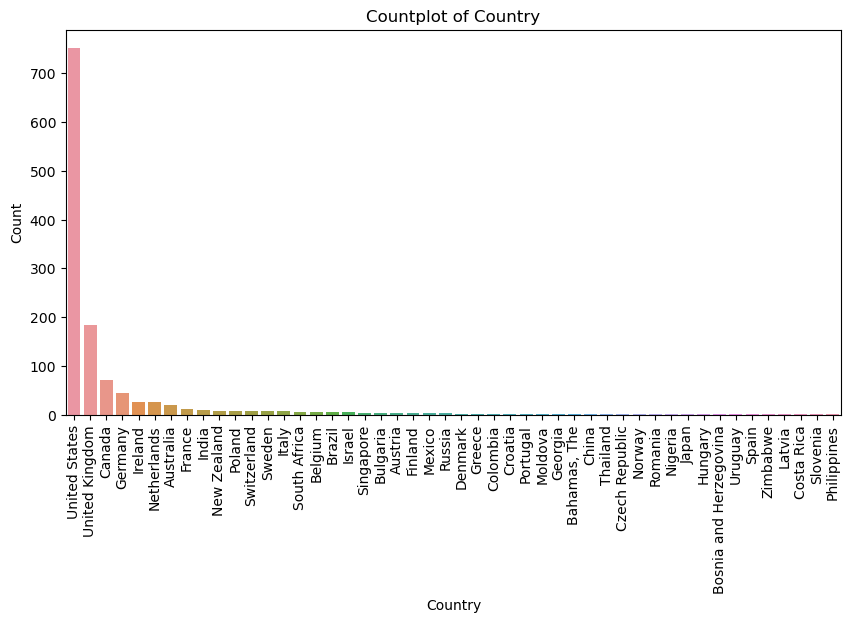
\includegraphics[width=15cm, height=9cm]{images/countries.png}
    \caption{Count plot of Country}
\end{wrapfigure}

\twocolumn
In order to provide better human-readability, summary statistics will be shown in their primary form (before encoding). Detailed statistics for every feature are included in the appendix section.

I decided to divide the features into following categories:

\subsubsection{\textbf{Personal info}}
The rounded average age is equal 32.03.\\

\begin{figure}[H]
    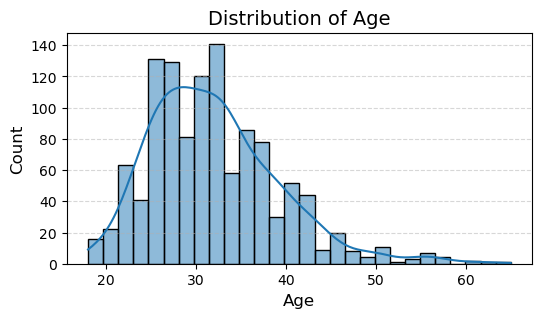
\includegraphics[width=0.48\textwidth]{age-distribution}
    \caption{Age distribution}
\end{figure}

\begin{figure}[H]
    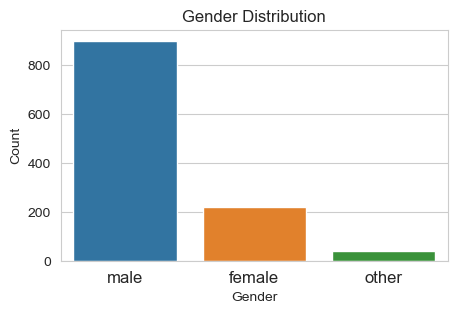
\includegraphics[width=0.48\textwidth]{gender-distribution}
    \caption{Gender distribution}
\end{figure}
The survey findings reveal a higher representation of males, mirroring the greater male presence observed in tech companies.\\ 

\subsubsection{\textbf{Workplace environment}}
Most of the respondents weren't self-employed. Predominantly they didn't work remotely and their company belonged to tech industry.\\

\subsubsection{\textbf{Care options}}
The main conclusion from this part of the survey is that generally people are unaware about their care options situation at work. Moreover employers tend to pay little attention to providing resources to learn more. Described stigma may contribute to detrimental effects on ones mental well-being.\\

\subsubsection{\textbf{Attitudes towards mental health}}
Generally people tend to be more concerned about their mental than physical health. Surprisingly, respondents prefer to discuss their psychological problem with their supervisors, rather than with coworkers.\\  

\subsubsection{\textbf{Mental health state}}
From chart below we can conclude that feature 'treatment' and 'work\_interfere' are strongly correlated. People who seek treatment tend to be more influenced by mental health conditions at work. Moreover, individuals who did not seek treatment for mental health issues predominantly had values of 'Never' or 'Unknown' in the 'work\_interfere' column. Therefore 'Unknown' and 'Never' were encoded with the same value - 0. In further analysis, a new output variable will be introduced: 'treatment\_work\_interfere\_product'.
\begin{figure}[h]
    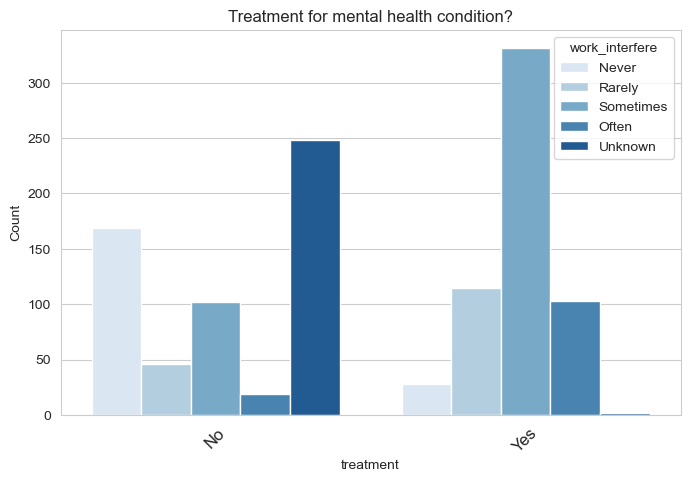
\includegraphics[width=0.48\textwidth]{images/treatment-work-interfere.png}
    \caption{'Work\_interfere' and 'treatment' chart}
\end{figure} 

\section{Experiments}
To discern the pivotal factors influencing the output variables: 'treatment', 'work\_interfere' and 'treatment\_work\_interfere\_product' ('treatment' * 'work\_interfere), I utilized the following techniques:
\begin{enumerate}
    \item Correlation matrix analysis
    \item Principal component analysis (PCA)
    \item Linear regression
\end{enumerate}

Analyzed models were created based on estimators available in scikit-learn.

\subsection{Correlation matrix analysis}
To enhance readability, only the highest correlations with outcome variables (excluding correlations with themselves) are presented in tables \ref{tab:top-corr-treatment}, \ref{tab:top-corr-work-interfere}, \ref{tab:top-corr-prod}: 

\begin{table}[h]
\centering
\begin{tabular}{|l|l|}
\hline
\textbf{Feature} & \textbf{Importance} \\ \hline
family\_history  & 0.384161            \\ \hline
care\_options    & 0.235402            \\ \hline
gender\_female   & 0.185874            \\ \hline
obs\_consequence & 0.159074            \\ \hline
benefits         & 0.138294            \\ \hline
\end{tabular}
\caption{Top correlations with 'treatment'}
\label{tab:top-corr-treatment}
\end{table}
\begin{table}[H]
\centering
\begin{tabular}{|l|l|}
\hline
\textbf{Feature}            & \textbf{Importance} \\ \hline
family\_history             & 0.334235            \\ \hline
mental\_health\_consequence & 0.196258            \\ \hline
obs\_consequence            & 0.177886            \\ \hline
care\_options               & 0.144964            \\ \hline
leave                       & 0.129800            \\ \hline
\end{tabular}
\caption{Top correlations with 'work\_interfere'}
\label{tab:top-corr-work-interfere}
\end{table}
\begin{table}[H]
\centering
\begin{tabular}{|l|l|}
\hline
\textbf{Feature}            & Importance \\ \hline
family\_history             & 0.356483   \\ \hline
care\_options               & 0.203670   \\ \hline
obs\_consequence            & 0.182370   \\ \hline
gender\_female              & 0.163761   \\ \hline
mental\_health\_consequence & 0.140258   \\ \hline
\end{tabular}
\caption{Top correlations with 'treatment\_work\_interfere\_product'}
\label{tab:top-corr-prod}
\end{table}

\subsection{Principal component analysis (PCA)}
The second method used in the analysis was the PCA. After conducting multiple iterations of this method with different numbers of components and evaluating their results, I discovered that PCA1 and PCA2 exhibited the highest accuracy in terms of explained variance. As a result, in order to provide better clarity in the report only those components will be presented.\\
\vspace{0.2cm}\\
Explained variance for PC1 = 0.51373783.\\
Explained variance for PC2 = 0.45604862.

\begin{table}[h]
\centering
\begin{tabular}{|l|l|}
\hline
\textbf{Feature} & \textbf{Importance} \\ \hline
treatment        & 0.480958            \\ \hline
family\_history   & 0.376527            \\ \hline
gender\_female    & 0.305439            \\ \hline
benefits         & 0.268926            \\ \hline
care\_options     & 0.267652            \\ \hline
\end{tabular}
\caption{Most important features for PC1}
\label{tab:pc1}
\end{table}

\begin{table}[h]
\centering
\begin{tabular}{|l|l|}
\hline
\textbf{Feature}            & \textbf{Importance} \\ \hline
mental\_health\_consequence & 0.378170            \\ \hline
leave                       & 0.191418            \\ \hline
phys\_health\_consequence   & 0.169851            \\ \hline
work\_interfere             & 0.115581            \\ \hline
obs\_consequence            & 0.114568            \\ \hline
\end{tabular}
\caption{Most important features for PC2}
\label{tab:pc2}
\end{table}

\begin{figure}[h]
    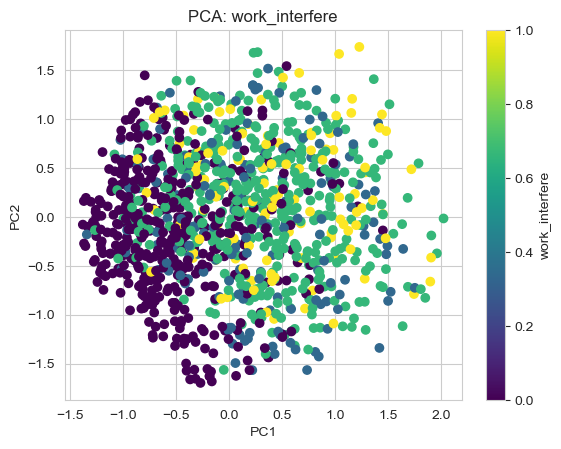
\includegraphics[width=0.45\textwidth]{images/pca-work-interfere.png}
    \centering
    \caption{PCA chart: work\_interfere}
\end{figure}
\begin{figure}[h]
    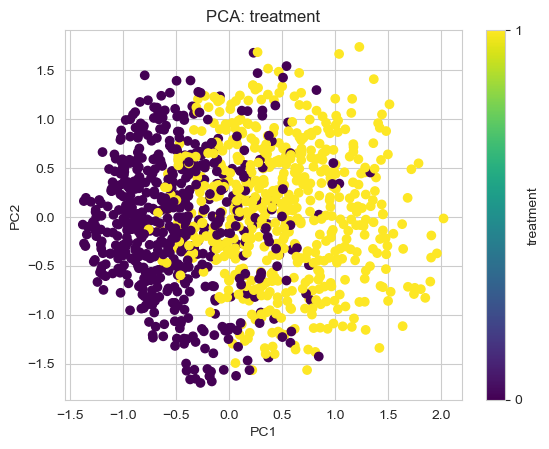
\includegraphics[width=0.45\textwidth]{images/pca-treatment.png}
    \centering
    \caption{PCA chart: treatment}
\end{figure}
\begin{figure}[H]
    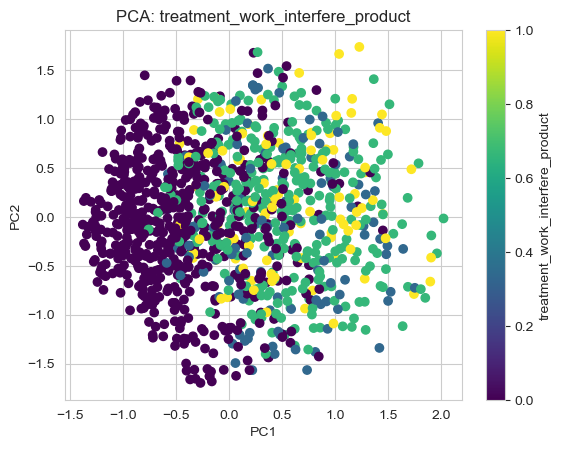
\includegraphics[width=0.45\textwidth]{images/pca-product.png}
    \centering
    \caption{PCA chart: treatment\_work\_interfere\_product}
\end{figure}

\subsection{Linear regression analysis}
All data used for linear regression is divided into training and testing data in a 75:25 ratio, with a random seed set to 13 to ensure consistent data sampling.\\
As a measure of model accuracy, r-squared score will be presented in table \ref{tab:r-squared-scores}.

\begin{table}[h]
\centering
\begin{tabular}{|l|l|}
\hline
\textbf{Feature}                    & \textbf{R-squared score} \\ \hline
work\_interfere                     & 0.1961795217360064       \\ \hline
treatment                           & 0.16670596803757243      \\ \hline
treatment\_work\_interfere\_product & 0.15178530861513928      \\ \hline
\end{tabular}
\caption{R-squared score for every model}
\label{tab:r-squared-scores}
\end{table}

\subsubsection{\textbf{work\_interfere}}
Most important features for determining work\_interfere in this model are: family\_history, mental\_health\_consequence, coworkers, care\_options and obs\_consequence.
\begin{figure}[H]
    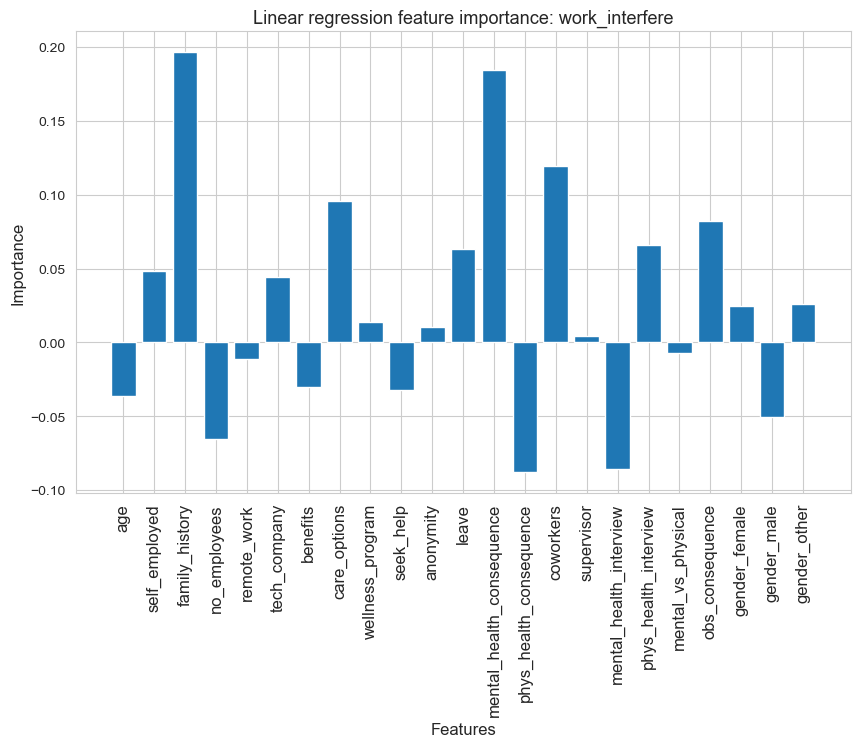
\includegraphics[width=0.5\textwidth]{images/lin-reg-work-interfere.png}
    \centering
    \caption{Linear regression feature importance: work\_interfere}
\end{figure}

\subsubsection{\textbf {treatment}}
Most important features for determining treatment in this model are: family\_history, coworkers, age, care\_options and mental\_health\_consequence.
\begin{figure}[H]
    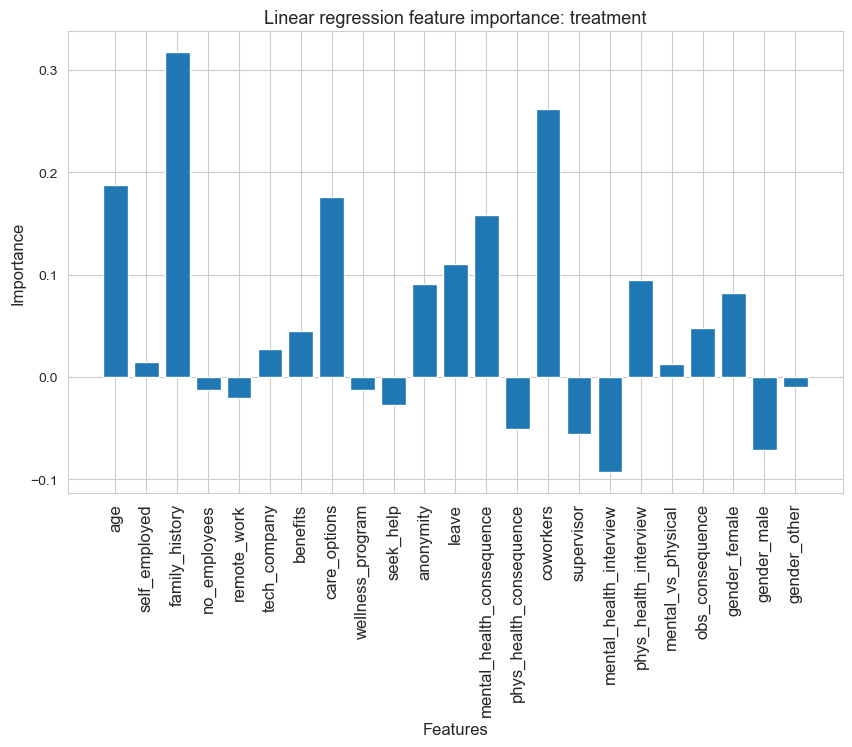
\includegraphics[width=0.5\textwidth]{images/lin-reg-treatment.png}
    \centering
    \caption{Linear regression feature importance: treatment}
\end{figure}

\subsubsection{\textbf{work\_interfere}}
Most important features for determining treatment\_work\_interfere\_product in this model are: family\_history, coworkers, mental\_health\_consequence, care\_options and phys\_health\_interview.
\begin{figure}[H]
    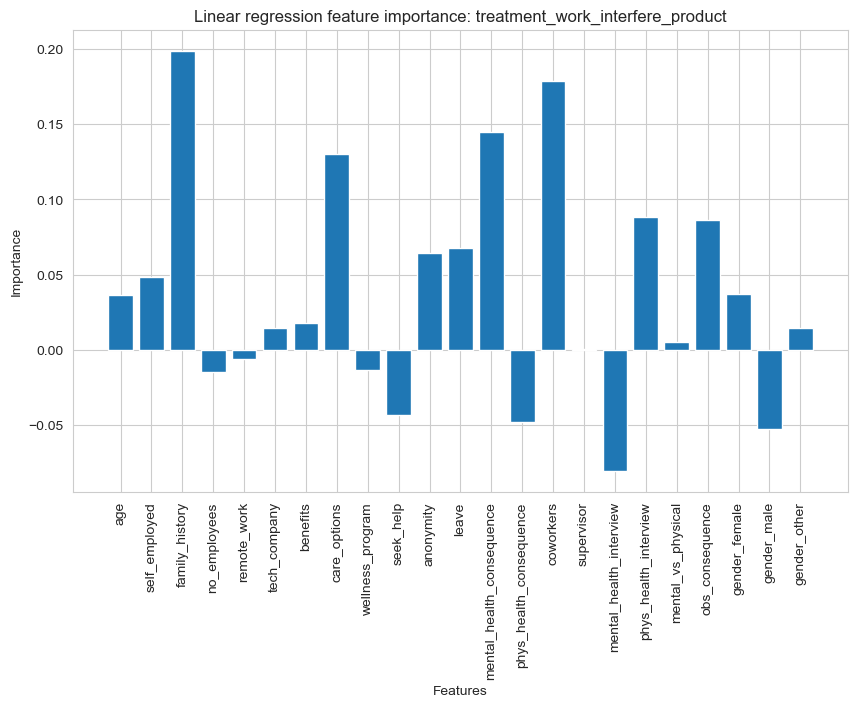
\includegraphics[width=0.5\textwidth]{lin-reg-product.png}
    \centering
    \caption{Linear regression feature importance: treatment\_work\_interfere\_product}
\end{figure}

\section{Conclusions}
Despite the fact that experiments accuracy was quite underwhelming (relatively low R-squared score in linear regression model (about 20\%) and medium  explained variance in PCA (about 50\%)), the outcomes were notably similar across all of them.\\

For every conducted experiment the strongest predictor for every output feature was family history of mental illness. This implies a strong genetic correlation or the impact family environment has on ones psychological state.\\

Secondly, the feature that appeared in every top 5 most important features was the awareness of care options provided by the employer. It suggests that when employees are well informed about available mental health resources they are more likely to seek treatment when needed. Without a doubt, this can be applied only when an appropriate program is already led. Therefore employers should emphasize this topic more often. \\

From the regression model, it can be concluded that employees who suffer from psychological problems are more prone to discuss it with their coworkers rather than with their supervisors.\\

Surprisingly, women generally tended to seek help more willingly than men.\\

Additionally, the feature indicating potential negative consequences of discussing a mental health issue with one's employer exhibits a strong positive correlation with the feature representing the extent to which an individual's mental state interferes with their work (work\_interfere).\\

Lastly, features describing workplace environment did not play a significant role in determining respondents mental state.\\

Summing up, it is vital for company's management to encourage employees to seek treatment for mental health problems and reduce stigma associated with it. Increasing awareness concerning that topic is also essential. Finally, employers could improve communication with their employees in order to reduce the amount of detrimental impact work has on their mental state.  

\bibliographystyle{IEEEtran}
\bibliography{references}

\newpage
\onecolumn
\section{Appendix}
\begin{figure}[h]
    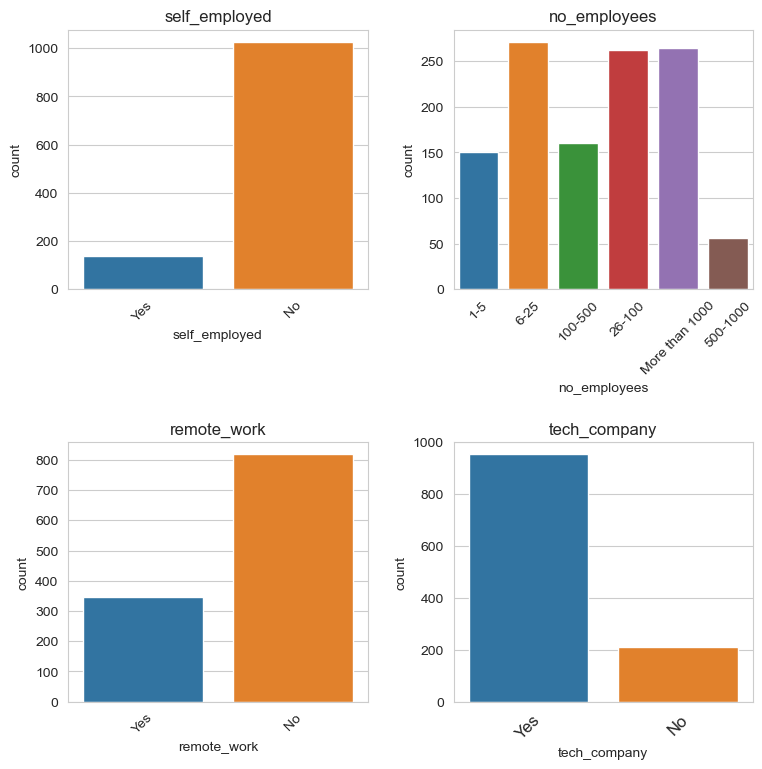
\includegraphics[width=0.75\textwidth]{images/workplace-environment.png}
    \centering
    \caption{Basic statistics for worplace environment features}
\end{figure}
\begin{figure}
    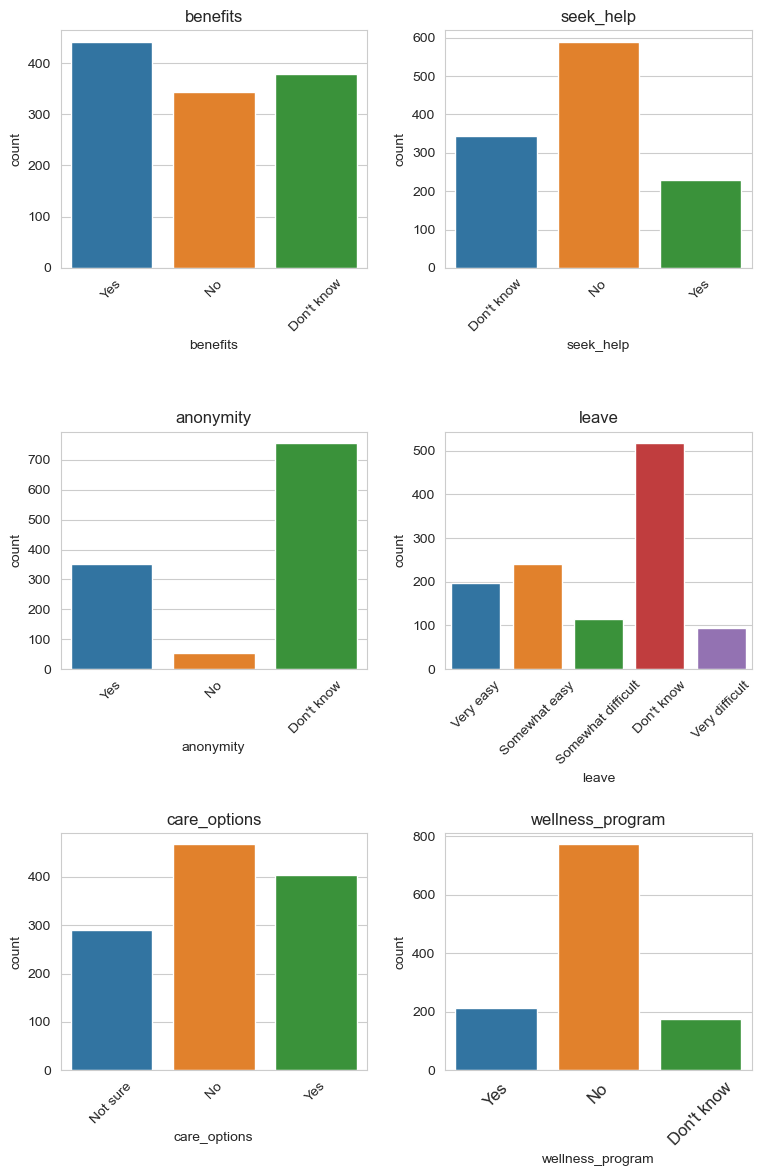
\includegraphics[width=0.75\textwidth]{images/care-options.png}
    \centering
    \caption{Basic statistics for care options features}
\end{figure}
\begin{figure}
    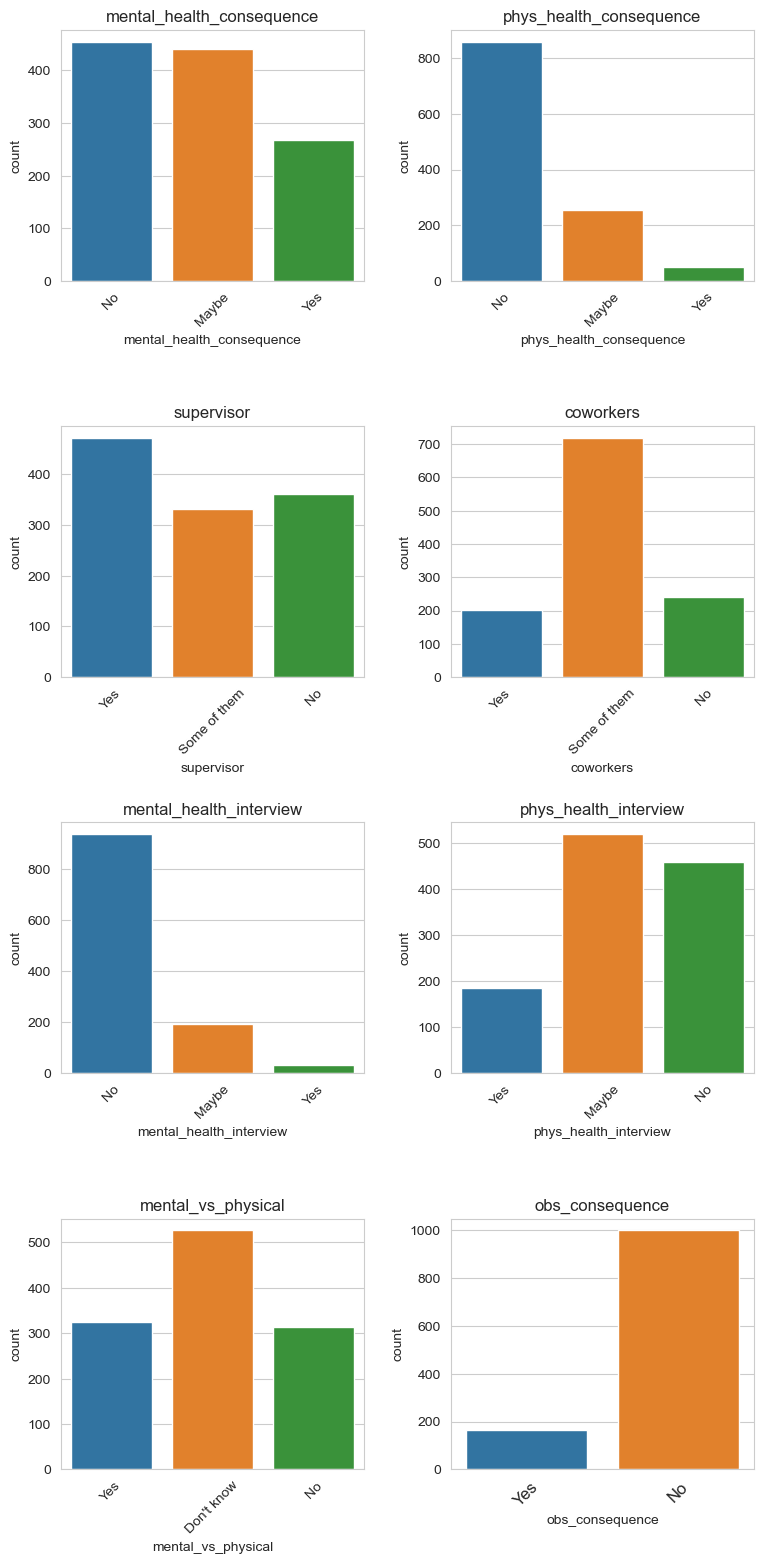
\includegraphics[width=0.6\textwidth]{images/attitude.png}
    \centering
    \caption{Basic statistics for attitude features}
\end{figure}
\begin{figure}
    \centering
    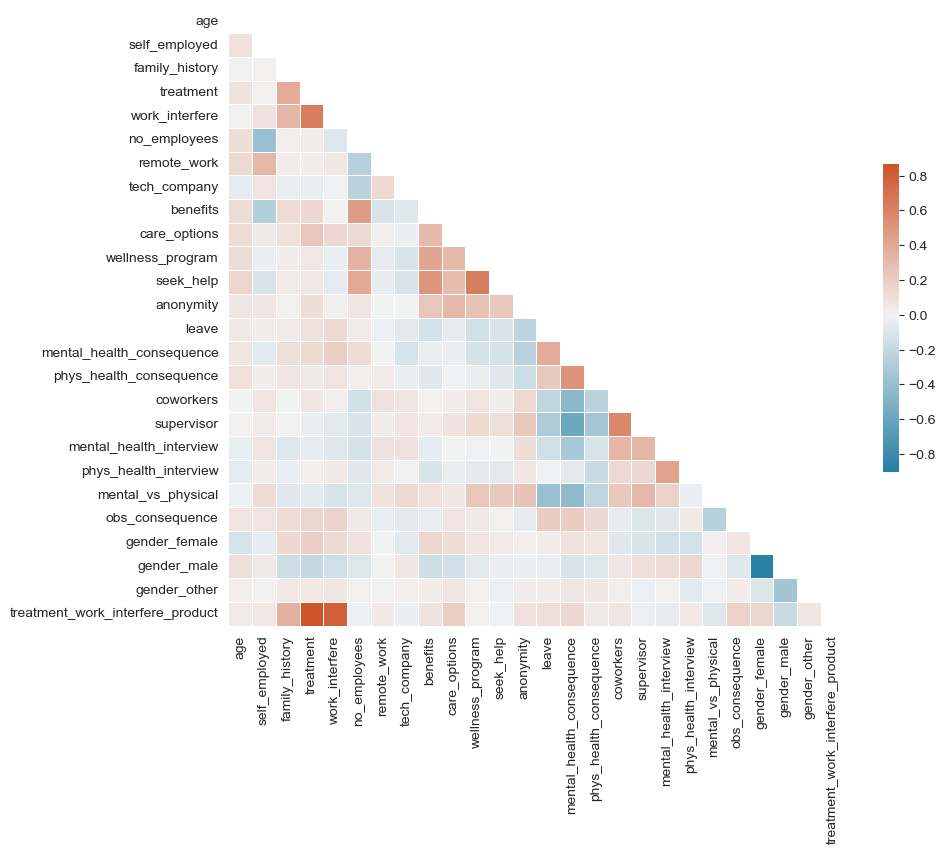
\includegraphics[width=\textwidth]{images/corr-matrix.png}
    \caption{Correlation matrix}
\end{figure}


\end{document}

